The dataset of our choice is managed by the University of California San Diego (UCSD) and is presented in this \href{https://nijianmo.github.io/amazon/index.html}{\color{blue}\underline{website}}.
It is composed of multiple collections of documents, each one containing some reviews, registered between the 1996 and 2018, about a specific kind of products sold on Amazon. 
This fact makes the dataset suitable for our purposes, since it contains a lot of reviews but also would make it possible to filter the reviews by product category, allowing to eventually focus the analysis on a specific kind of goods.

In particular, in the website cited above, are provided 2 versions of the same datasets:
\begin{itemize}
    \item \textit{5-core}: this is a reduced version of the original, complete dataset, in which are included at least 5 of the most representative reviews per product and user
    \item \textit{ratings only}: in this version of the dataset only information about the user, the product, the rating and the timestamp of pubblication time is kept for each review
\end{itemize}
While the second version of the dataset contains an higher amount of reviews, we decided to use the first one since it contained more interesting fields.

\begin{figure}[H]
    \centering
    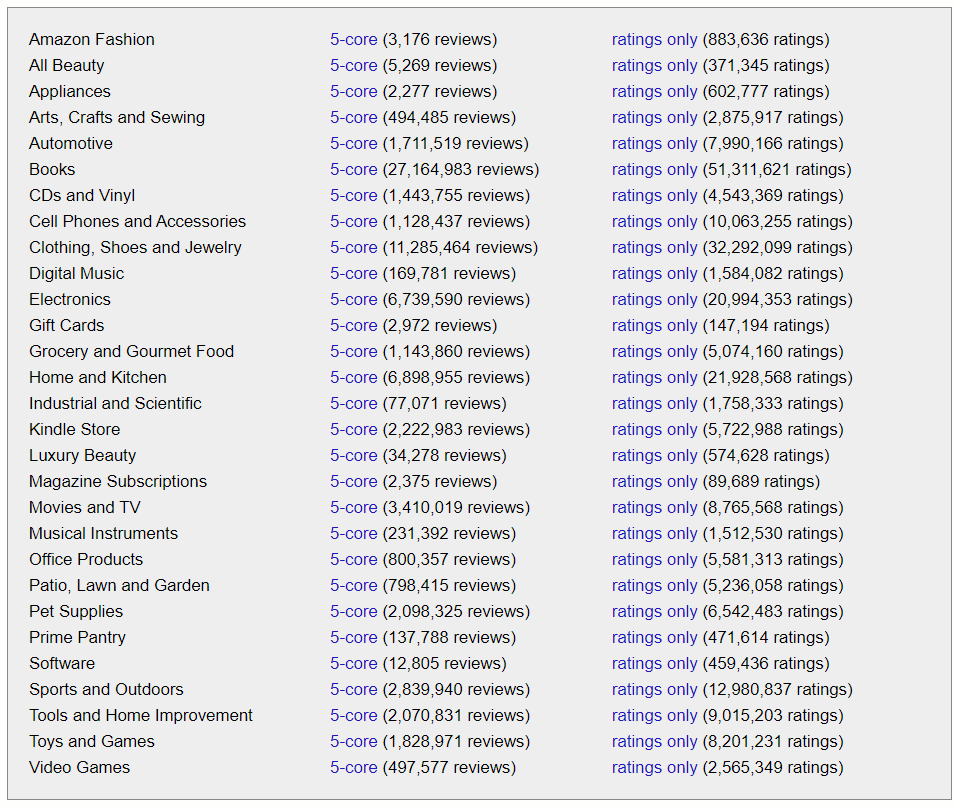
\includegraphics[scale=0.5]{Images/collections.png}
    \caption{List of the collections provided by the dataset}
\end{figure}

Among all the available collections, we've decided to use the one about \textbf{Digital Music} (which can be retrieved at this \href{https://jmcauley.ucsd.edu/data/amazon_v2/categoryFilesSmall/Digital_Music_5.json.gz}{\color{blue}\underline{link}}) since this file includes a suitable number of datapoints (169.781) while still containing an interesting amount of attributes per document.
Specifically, the documents inside the selected collection have the following shape:
\begin{verbatim}
{
    "image": ["https://images-na.ssl-images-amazon.com/images/..."], 
    "overall": 5.0, 
    "vote": "2",
    "verified": true, 
    "reviewTime": "01 8, 2015", 
    "reviewerID": "A36GE53TK8V94L", 
    "asin": "B000T1EJ0W", 
    "style": {"Format:": "MP3 Music"}, 
    "reviewerName": "MysticWolf229", 
    "reviewText": "the theme song to the one and only movie that ...", 
    "unixReviewTime": 1420675200
}
\end{verbatim}
whose fields have the following meaning:
\begin{itemize}
    \item \textbf{image}: an array of URLs pointing to the images of the product review;
    \item \textbf{overall}: the rating of the product, a float number going from 1 to 5;
    \item \textbf{vote}: the number of people that found the review helpful, saved as a string;
    \item \textbf{verified}: a boolean value indicating whether the purchase of the product from the user making the review has been verified or not;
    \item \textbf{reviewTime}: the date of the review, saved in RAW date format as a string;
    \item \textbf{reviewerID}: the alphanumeric ID of the user who wrote the review;
    \item \textbf{asin}: acronym of Amazon Standard Identification Number, is the alphanumeric ID that represents a specific product;
    \item \textbf{style}: a subdocument containing additional data about the version of the product. In the case of this collection it just contains information about the format of the product, whose possible values will be retrieved with a suited query;
    \item \textbf{reviewerName}: a string containing the name of the user who wrote the review;
    \item \textbf{reviewText}: a string containing the text of the review;
    \item \textbf{summary}: a string containing a summary of the review;
    \item \textbf{unixReviewTime}: the date of the review in Unix epoch time format.
\end{itemize}